\documentclass[10pt]{report}
\usepackage{../style}

\begin{document}
\section{Topological Spaces and Bases (\S M12-13)}
\subsection{Topological Spaces}
\begin{definition}
  A \emph{topology} on a set $X$ is a collection $\ST$ of subsets of $X$ having the following properties:
  \begin{enumerate}[label={(\arabic*)}]
    \item $\varnothing$ and $X$ are in $\ST$.
    \item The union of any subcollection of $\ST$ is in $\ST$.
    \item The intersection of any finite subcollection of $\ST$ is in $\ST$.
  \end{enumerate}
  A set $X$ for which a topology $\ST$ has been specified is a \emph{topological space}, and any subset $U \subset X$ is open if $U \in \ST$.
\end{definition}

  Examples of this include the \emph{discrete topology}, where every subset is open, and the \emph{indiscrete} or \emph{trivial topology}, where only $\varnothing$ and $X$ are open.
  
  Another important (probably) example is the \emph{finite complement topology}:
  this is $(X,\ST_f)$, where $\ST_f$ is the collection of subsets $U \subset X$ such that $X - U$ is either finite or all of $X$.
  It's easy to check that $X$, $\emptyset$ work, so we note the following facts for an indexed family of nonempty elements $\{U_\alpha\} \subset \ST_f$:
  \[ X - \bigcup U_\alpha = \bigcap (X - U\alpha;) \]
  \[ X - \bigcap_{i=1}^n U_i = \bigcup_{i = 1}^n (X - U_i). \]
  From this, one can see that arbitrary unions and finite intersections work. 

\begin{definition}
  Suppose that $\ST$, $\ST'$ are topologies on $X$.
  If $\ST' \supset \ST$, then $\ST'$ is \emph{finer} than $\ST$ (and \emph{strictly finer} with a proper inclusion).
  The reverse inclusion implies $\ST'$ is \emph{coarser} than $\ST$.
  If either of these inclusions is true, then $\ST'$ is \emph{comparable} to $\ST$.
\end{definition}

Sometimes fully specifying the elements of a topology is difficult or annoying--like in algebra, one usually specifies a topology by a subcollection of open sets which generate the whole thing.

\subsection{Bases}
\begin{definition}
  If $X$ is a set, a \emph{basis} for a topology on $X$ is a collection $\SB$ of subsets of $X$ (called \emph{basis elements}) such that
  \begin{enumerate}[label={(\arabic*)}]
    \item For each $x \in X$, there exists some $B \in \SB$ with $x \in B$.
    \item If $x \in B_1 \cap B_2$, then there exists $B_3 \in \SB$ with $x \in B_3 \subset B_1 \cap B_2$.
  \end{enumerate}
  
  If $\SB$ satisfies these conditions, then we define the \emph{topology $\ST$ generated by $\SB$} by the following:
  $U \subset X$ is open if, for each $x \in U$, there is some $B \in \SB$ with $x \in B \subset U$.
\end{definition}

  We will show that this is a topology.
  Note that $\varnothing$ satisfies the condition for openness vacuously, and all $x \in X$ are contained in a basis element by hypothesis, so $X$ is open as well.
  All that's left is that unions and finite intersections work.

  Suppose $\{U_\alpha\} \subset \ST$ is a collection of open sets.
  Then, for any element $x \in \bigcap U_\alpha$, $x \in U_\alpha$ for some $\alpha$; choose $x \in \SB$ with $x \in B \subset U_\alpha$ and note that this is also in the union.
  For the intersection, we will prove the intersection of two and use induction; suppose $U,V \in \ST$.
  Then, for any $x \in U \cap V$, choose $B_1,B_2 \in \ST$ containing $x$ so that $B_1 \subset U$ and $B_2 \subset V$; then, by definition, there exists a $B_3 \subset B_1 \cap B_2$ with $x \in B_3 \subset \ST$, giving openness.
  Induction is straightforward.

  \begin{lemma}
    Let $X$ be a set and let $\SB$ be a basis for a topology $\ST$ on $X$.
    Then $\ST$ is the collection of all unions of elements of $\SB$.
  \end{lemma}
  \begin{proof}
    That $\ST$ includes all unions is straightforward from the fact that $\ST$ is a topology.
    To show that any $U \in \ST$ is a union of elements, choose for each $x \in U$ some $B_x \in \SB$ such that $x \in B_x \subset U$.
    Then $U = \bigcup B_x$, so $U$ is a union of elements of $\SB$.
  \end{proof}

  There is one significant, potentially counter-intuitive fact to note about bases:
  the representation of any open subset as a union of basis elements is not unique.
  Topological bases seem similar to the algebraic notion of a spanning set or generating set.

  \begin{lemma}
    Let $X$ be a topological space.
    Suppose that $\SC$ is a collection of open sets of $X$ such that, for each $X$ of $X$ and each $x \in U$, there is an element $C \in \SC$ such that $x \in C \subset U$.
    Then $\SC$ is a basis for the topology of $X$.
  \end{lemma}
  \begin{proof}
    First we check that $\SC$ is a basis.
    The first condition is easy; since $X$ is open, there is an element $C \in \SC$ with $x \in C \subset X$.
    To show the intersection property, take any $x \in C_1 \cap C_2$, where $C_i \in \SC$.
    Then, since $C_1 \cap C_2$ is open, there exists an element $C_3 \in \SC$ with $x \in C_3 \subset C_1 \cap C_2$.

    Suppose $\ST$ is the set of open sets on $X$ and $\ST'$ is generated by $\SC$.
    Note that, for any $U \subset \ST$ with $x \in U$, there exists an element $C \in \SC$ with $x \in C \subset U$, so $\ST'$ is finer than $\ST$.
    Conversely, if $W \in \ST'$, then $W$ is a union of elements of $\SC$, which are each open, so $W$ is open and $\ST$ is finer than $\ST'$, giving $\ST = \ST'$.
  \end{proof}

  \begin{lemma}
    Let $\SB$ and $\SB'$ be bases for the topologies $\ST$ and $\ST'$ on $X$.
    Then the following are equivalent:
    \begin{enumerate}[label={(\arabic*)}]
      \item $\ST'$ is finer than $\ST$
      \item For each $x \in X$ and each basis element $B \in \SB$ containing $x$, there is a basis element $B' \in \SB'$ such that $x \in B' \subset B$.
    \end{enumerate}
  \end{lemma}
  \begin{proof}
    $(2) \implies (1)$. Suppose $U \in \ST$.
    Then for each $x \in U$, there is a $B_x \in \ST$ containing $x$ as a subset of $U$.
    By hypothesis, there exists a $B_x' \in \ST'$ with $x \in B_x' \subset B_x \subset U$, so $U$ is the union of elements of $\SB'$ and $U \in \ST'$.

    $(1) \implies (2)$. Suppose $U \in \ST$.
    Then, for each $x \in U$ and $B \in \SB$ containing $x$, by condition $(1)$ and the definition of generation, $B \in \ST'$; since $\ST'$ is generated by $\SB'$, there is an element $B' \in \SB'$ such that $x \in B' \subset B$.
  \end{proof}
  
  We will move on to our first serious examples of topological spaces:
  \begin{definition}
    If we denote the collection of all open intervals on the real line $\SB$, 
    \[ \prn{a,b} = \cbr{x \mid a < x < b }, \]
    the topology generated by $\SB$ is the \emph{standard topology} on the real line.
    This is the topology assumed for $\RR$ unless otherwise specified.

    If $\SB'$ is the half open intervals, we will call the topology generated by $\SB'$ the \emph{lower limit topology} on $\RR$; denote $\RR$ with this topology by $\RR_l$.

    If we let $K$ be the set of numbers of the form $1/n$ and let $\SB''$ be the collection of all open intervals $(a,b)$ and sets of the form $(a,b) - K$, we call the topology generated by $\SB''$ the \emph{K-topology} on $\RR$, denoted by $\RR_k$.
  \end{definition}

  \begin{lemma}
    The topologies of $\RR_l$ and $\RR_k$ are strictly finer than the standard topology on $\RR$, but are not comparable with one another.
  \end{lemma}
  \begin{proof}
    Let $\ST$, $\ST_l$, and $\ST_k$ be the topologies on $\RR$, $\RR_l$, and $\RR_k$.
    To show that $\ST_l$ is finer than $\ST$, take any $(a,b) \in \ST$ and $x \in (a,b)$; then $[x,b)$ contains $x$ and lies in $(a,b)$.
    However, no $(c,d) \subset [x,b)$ contains $x$, so $\ST_l \supsetneq \ST$.
    To show that $\ST_k$ is finer than $\ST$, any $(a,b) \in \ST$ has $(a,b) \in \ST_k$ by construction.
    However, $(-1,1) - K$ has no subset in $\ST$ containing 0, giving $\ST_k \supsetneq \ST$.
  
    To see that these are not comparable, use a similar argumen to before.
    There is no $(c,d) - K \subset [x,b)$ containing $x$, and there is no $[a,b) \subset (-1,1)-k$ contining $0$.
  \end{proof}

  One last basic\footnote{This was intended to be a really bad pun} definition:
  \begin{definition}
    A subbasis $\CS$ for a topology on $X$ is a collection of subsets of $X$ whose union equals $X$.
    The \emph{topology generated by the subbasis $\CS$} is defined to be the collection $\ST$ of all unions of finite intersections of the elements of $\CS$.
  \end{definition}

  We'll check that $\ST$ is a topology.
  By an earlier lemma, it suffices to show that the collection of finite intersections of $\CS$ is a basis.
  Given $x \in X$, it belongs to an element of $\CS$ and hence an element of $\SB$, giving the first condition.
  To show the second condition, let $B_1 = S_1 \cap \dots \cap S_m$ and $B_2 = S_1' \cap \dots \cap S_n'$ be any two elements of $\SB$; then $B_1 \cap B_2 = S_1 \cap \dots \cap S_m \cap S_1' \cap \dots \cap S_n' \in \SB$, making $\SB$ a basis.
 

\newpage
\section{Closed Sets and Limit Points}
I'll defer talking about particular examples until later.
Refer to ``Basic Examples of Topological Spaces'' at the end of the chapter for definitions of order, product, subspace topologies, etc.
First I'll cover closed sets, limit points, and the Hausdorff axiom.

\subsection{Closed Sets}
We say a subset of a topological space is \emph{closed} if its complement is open.
\begin{theorem}
  Let $X$ be a topological space.
  Then the following conditions hold:
  \begin{enumerate}[label={(\arabic*)}]
    \item $\varnothing$ and $X$ are closed.
    \item Arbitrary intersections of closed sets are closed.
    \item Finite unions of closed sets are closed.\footnote{Use DeMorgan's Law}\qed
  \end{enumerate}
\end{theorem}

Note: while this is rarely done, a collection of closed sets satisfying these theorems can be used to specify a topology rather than open sets.

\begin{theorem}
  Let $Y$ be a subspace of $X$.
  Then a set $A$ is closed in $Y$ iff it is the intersection of a closed set of $X$ with $Y$.
\end{theorem}
\begin{proof}
  Suppose that $A = Y \cap C$ for some $C$ which is closed in $X$.
  Then there exists some $U = X - C$ which is open in $X$, and for which
  \[
    U \cap Y = Y - C \cap Y = Y - A
  \]
  is open in $Y$, meaning $A$ is closed in $Y$.
  
  Conversely, suppose $A$ is closed in $Y$.
  Then $Y - A$ is open, so there exists an open $U$ such that
  \[
    U \cap Y = Y - A
  \]
  and $X - U$ is closed in $X$, so that $A = (X - U) \cap Y$, the intersection of $Y$ and a closed set of $X$.\footnote{Ahh this proof is messy as hell, but the idea is there}
\end{proof}

\begin{theorem}
  Let $Y$ be a subspace of $X$.
  If $A$ is closed in $Y$ and $Y$ is closed in $X$, then $A$ is closed in $X$.\footnote{The proof was ``left to the reader,'' but this is an obvious finite intersection on closed sets in $X$ using the previous theorem.}\qed
\end{theorem}

\subsection{Closure and Interior of a Set}
We'll talk about the closure and interior, functionally the largest open subset and smallest closed subset.
\begin{definition}
  Given a subset $A$ of a topological space $X$, the \emph{interior} of $A$ is the union of all open sets contained in $A$, and the \emph{closure} of $A$ is the intersection of all closed sets containing $A$.
\end{definition}

Note the following inclusion, with $\Int A = A$ if open and $A = \bar A$ if closed:
\[
  \Int A \subset A \subset \bar A.
\]
In the situation where $A$ is a subset of $Y$ which is a subspace of $X$, we'll use care, and generally define the closure $\bar A$ as the closure of $A$ in $Y$.
More on this follows:

\begin{theorem}
  Let $Y$ be a subspace of $X$,
  let $A$ be a subset of $Y$,
  and let $\bar A$ denote the closure of $A$ in $X$.
  Then the closure of $A$ in $Y$ equals $\bar A \cap Y$.
\end{theorem}
\begin{proof}
  Denote the closure of $A$ in $Y$ as $B$.
  Since $\bar{A}$ is closed, $\bar{A} \cap Y$ is closed and contains $A$;
  then, $B \subset \bar A \cap Y$ by property of the intersection.

  On the other hand, since $B$ is closed in $Y$, $B = C \cap Y$ for some $C$ closed in $X$;
  $C$ is a closed set of $C$ containing $A$;
  then $\bar{A} \subset C$, so $(\bar A \cap Y) \subset (C \cap Y) = B$
\end{proof}

We'll write that a set $A$ \emph{intersects} a set $B$ if the intersection $A \cap B$ is nonempty.

\begin{theorem}
  Let $A$ be a subset of the topological space $X$.
  \begin{enumerate}[label={(\alph*)}]
    \item Then $x \in \bar A$ iff every open set $U$ containing $x$ intersects $A$.
    \item Supposing the topology of $X$ is given by a basis, then $x \in \bar A$ iff every basis element $B$ containing $x$ intersects $A$.
  \end{enumerate}
\end{theorem}
\begin{proof}
  We'll prove (a) using contraposition;
  if $x \notin \bar{A}$, then $U = X-\bar{A}$ is an open set in $X$ which contains $x$ and doesn't intersect $A$.
  If $U$ contains $x$ and doesn't intersect $\bar{A}$, then $X - U$ is a closed set containing $A$; then $X - U$ must contain $\bar A$, so $x \notin \bar A$.

  The rest follows from this.
  If not every basis element containing $x$ intersects $A$, then by (a), $x \notin \bar A$.
  If every basis element containing $x$ intersects $\bar A$, then so does every open set containing $x$ by definition of bases (each open set containing $x$ contains a basis element containing $x$).
\end{proof}

We'll write ``$U$ is an open set containing $x$'' as ``$U$ is a \emph{neighborhood} of $x$.''
Using this, we can rewrite the previous theorem as ``if $A$ is a subset of a topological space $X$, then $x \in \bar{A}$ iff every neighborhood of $X$ intersects $A$.''

\subsection{Limit Points}
We seek another way of describing closures.
\begin{definition}
  If $A$ is a subset of a topological space $X$, and $x$ is a point of $x$, we call $x$ a \emph{limit point} (or cluster point, point of accumulation) if every neighborhood of $x$ intersects $A$ in some point other than $x$ itself.
  In other words, $x$ is a limit point of $A$ if it belongs to the closure of $A - \cbr{x}$.
\end{definition}

\begin{theorem}
  Let $A$ be a subset of the topological space $X$ and let $A'$ be the set of all limit points of $A$. Then
  \[
    \bar A = A \cup A'.
  \]
\end{theorem}
\begin{proof}
  If $x \in A'$, every neighborhood of $x$ intersects $A$, so $A' \subset \bar A$.
  Furthermore, by definition, $A \subset \bar A$, so $A \cup A' \subset \bar A$.

  Let $x \in \bar A$; if $x \in A$ then $x \in A \cup A'$ trivially.
  Otherwise, every neighborhood of $x$ intersects $A$ at a point other than $x$, meaning $x \in A'$ so $x \in A \cup A'$ as desired.
\end{proof}
\begin{corollary}
  A subset of a topological space is closed iff it contains its limit points.\qed
\end{corollary}

\subsection{Hausdorff Spaces}
Note: not all topological spaces have closed one-point sets, and not all convergent sequences in general topological spaces converge to a unique point.
Examples of this come from the topology on $\cbr{a,b,c}$ indicated in figure 17.3 of Munkres.
We get rid of these with an extra axiom:
\begin{definition}
  A topological space $X$ is classed a \emph{Hausdorff space} if, for each pair $x_1,x_2$ of distinct points of $X$, there exist neighborhoods $U_1$ and $U_2$ of $x_1$ and $x_2$ which are disjoint.
\end{definition}

\begin{theorem}
  Every finite point set in a Hausdorff space is closed.
\end{theorem}
\begin{proof}
  It's sufficient to show that one-point sets are closed.
  Consider the one point set $\cbr{x_1}$ and any other element $x_2 \in X$.
  By definition, there is a neighborhood $U_2$ of $x_2$ which is disjoint from a neighborhood of $x_1$, which must contain $x_1$, i.e. $x_1 \notin U_2$; then $x_2$ isn't a limit point of $\cbr{x_1}$, so it is closed.
  Finite unions of closed one-point sets give the theorem.
\end{proof}

In fact, that finite-point sets are closed is weaker than the Hausdorff condition; we call this the \emph{$T_1$ axiom}.
In particular, $\RR$ with the finite complement topology is not a Hausdorff space, but it satisfies the $T_1$ axiom by construction.
We won't use the $T_1$ axiom very much, but it's important now:

\begin{theorem}
  Let $X$ be a space satisfying the $T_1$ axiom and let $A \subset X$.
  Then $x$ is a limit point of $A$ iff every neighborhood of $x$ contains infinitely many points of $A$.
\end{theorem}
\begin{proof}
  If every neighborhood of $x$ intersects $A$ at infinitely many points then $x$ is clearly a limit point of $A$.

  Suppose that $x \in X$ and suppose some neighborhood $U$ of $x$ intersects $A$ in finitely many points.
  Let $U \cap (A - \{x\}) = \cbr{x_1,\dots,x_n}$;
  then $X - \cbr{x_1 \dots x_n}$ is an open set of $X$ and
  \[ U \cap (X - \cbr{x_1,\dots,x_n})\]
  is a neighborhood of $x$ which doesn't intersect $A$.
  Hence $x$ is not a limit point of $A$ and the theorem follows.
\end{proof}

\begin{theorem}
  Let $x_n$ be a sequence of points in a Hausdorff space $X$ which converges; then $x_n$ converges to one point.
\end{theorem}
\begin{proof}
  Suppose $x_n \rightarrow x$ and $y \neq x$.
  Let $U$ and $V$ be disjoint neighborhoods of $x$ and $y$; then all but finitely many points of $x_n$ fall within $U$, so the same can't be true of $V$, and $x_n$ doesn't converge to $y$.
\end{proof}

\begin{theorem}
  The following examples are true:
  \begin{enumerate}[label={(\alph*)}]
    \item Every simply ordered set is a Hausdorff space in the order topology.
    \item The product of two Hausdorff spaces is a Hausdorff space.
    \item A subspace of a Hausdorff space is a Hausdorff space.
 \end{enumerate}
\end{theorem}
\begin{proof}
  Suppose $X$ is simply ordered with the order topology and $x,y \in X$.
  Without loss of generality, assume $x < y$; if there is an intermediate element $x < c < y$ then choose $(-\infty,c)$ and $(c,\infty)$ for disjoint neighborhoods; if no such element exists, then $(-\infty,y)$ and $(x,\infty)$ are disjoint open neighborhoods of $x$ and $y$ and the order topology is Hausdorff.

  Suppose $X$ and $Y$ are Hausdorff spaces and consider the product topology on $X \times Y$.
  Take any $x \times y , x' \times y' \in X \times Y$ distinct and neighborhoods $U,V,U',V'$ around those points with $U,U'$ if $x \neq x'$ and $V,V'$ disjoint if $y \neq y'$ (at least one of these is true).
  Then, $U \times V$ and $U' \times V'$ are disjoint neighborhoods of the points and the product topology is Hausdorff.

  Suppose $Y$ is a subspace of a Hausdorff space $X$, and suppose $x,y \in A$.
  Let $U,V$ be disjoint neighborhoods of $x,y$ in $X$;
  then $U \cap Y$ and $V \cap Y$ are disjoint neighborhoods of $x,y$ in $Y$ and the subspace topology is Hausdorff.
\end{proof}

\newpage
\section{Continuous Functions}
\subsection{Continuity of a Function}
\begin{definition}
  Let $X$ and $Y$ be topological spaces.
  A function $f:X \rightarrow Y$ is \emph{continuous} if, for each open $V \subset Y$, the set $f^{-1}(V) \subset X$ is open.
  We may say that $f$ is continuous relative to specific topologies on $X$ and $Y$.
\end{definition}

Note: this can be shown equivalently using only the open preimages of every basis or subbasis element.
A good non-example is the identity $f:\RR \rightarrow \RR_l$, for which the inverse image of the open set $[a,b)$ of $\RR_l$ is not an open set in $\RR$.
Note that the identity function $\RR_l \rightarrow \RR$ is continuous.

\begin{theorem}
  Let $X$ and $Y$ be topological spaces and let $f: X \rightarrow Y$.
  Then the following are equivalent:
  \begin{enumerate}[label={(\arabic*)}]
    \item $f$ is continuous.
    \item For every subset $A$ of $X$, $f(\bar A) \subset \overline{f(A)}$.
    \item For every closed set $B$ of $Y$, the set $f^{-1}(B)$ is closed in $X$.
    \item For each $x \in X$ and each neighborhood $V$ of $f(x)$, there is a neighborhood $U$ of $x$ such that $f(U) \subset V$.
  \end{enumerate}
  If (4) holds for the point $x \in X$, then we say that $f$ is \emph{continuous at $x$}.
\end{theorem}
\begin{proof}
  We'll show that $(1) \implies (2) \implies (3) \implies (1)$ and $(1) \implies (4) \implies (1)$.
  
  Suppose $f$ is continuous, and take some $x \in \bar A$.
  Take some neighborhood $V$ of $f(x)$; then $f^{-1}(V)$ is an open set of $X$ containing $x$, so it must intersect $A$ at some point $y$.
  Then $V$ intersects $f(A)$ at $f(y)$, meaning $f(x) \in \overline{f(A)}$ as desired.

  Suppose (2), let $B$ be a closed set of $Y$, and let $F = f^{-1}(B)$.
  Then $f(\bar{F}) \subset \bar{B} = B$, so that $x \in F$ for all $\bar F$; hence $F = \bar F$ and $F$ is closed.

  Suppose (3), and let $V$ be an open subset of $Y$.
  Then $f^{-1}(Y - V) = X - f^{-1}(V)$ is closed, meaning $f^{-1}(V)$ is open and $f$ is continuous.
 
  Suppose $f$ is continuous and take some $x \in X$ and neighborhood $V$ of $f(x)$.
  Since $f^{-1}(V)$ is open, there is some neighborhood $U$ of $x$ contained in it; then $f(U) \subset V$.

  Suppose (4), and let $V$ be an open set of $Y$.
  Then, for every $x \in f^{-1}(V)$, there exists an open neighborhood $U_x$ of $x$ with $f(U_x) \subset V$.
  Hence $f^{-1}(V) = \bigcup U_x$, meaning $f^{-1}(V)$ is open and $f$ is continuous.
\end{proof}

\subsection{Homeomorphisms}
\begin{definition}
  Let $X$ and $Y$ be topological spaces and let $f:X \rightarrow Y$ be a bijection.
  If $f$ and $f^{-1}$ are continuous, then $f$ is called a \emph{homeomorphism}.
  Equivalently, $f$ is a homeomorphism if $f(U)$ is open iff $U$ is open.
\end{definition}

We will call any property of a space $X$ that is expressed fully via the topology of $X$ a \emph{topological property} of $X$, and homeomorphism between $X$ and $Y$ yields the same topological property for $Y$.
This is similar to the algebraic structure of isomorphism.

Suppose $f:X \rightarrow Y$ is an injective continuous map between topological spaces.
Let $Z$ be the image set $f(X)$ considered as a subspace of $Y$; then $f':X \rightarrow Z$ is a bijection.
If $f'$ is a homeomorphism of $X$ with $Z$, then $f:X \rightarrow Y$ is a \emph{topological imbedding} or just an \emph{imbedding} of $X$ in $Y$.

\subsection{Constructing Continuous Functions}
\begin{theorem}
  Let $X,Y,Z$ be topological spaces.
  \begin{enumerate}[label={(\alph*)}]
    \item \emph{(Constant function)} If $f:X \rightarrow Y$ maps all of $X$ into a single point $y_0$ of $Y$, then $f$ is continuous.
    \item \emph{(Inclusion)} If $A$ is a subspace of $X$, the inclusion function $\iota: A \rightarrow X$ is continuous.
    \item \emph{(Composites)} If $f: X \rightarrow Y$ and $g:Y \rightarrow Z$ are continuous, then the map $g \circ f: X \rightarrow Z$ is continuous.
    \item \emph{(Restricting the domain)} If $f:X \rightarrow Y$ is continuous, and if $A$ is a subspace of $X$, then the restricted function $f \mid _A : A \rightarrow Y$ is continuous.
    \item \emph{(Restricting or expanding the range)} Let $f:X \rightarrow Y$ be continuous.
      If $Z$ is a subspace of $Y$ containing the image set $f(X)$, then $g:X \rightarrow Z$ obtained by restricting the range of $f$ is continuous.
      If $Z$ is a space having $Y$ as a subspace, then $h:X \rightarrow Z$ obtained by expanding the range of $f$ is continuous.
   \item \emph{(Local formulation of continuity)} The map $f:X \rightarrow Y$ is continuous if $X$ can be written as the union of open sets $U_\alpha$ such that $f \mid _{U_\alpha}$ is continuous for each $\alpha$.
  \end{enumerate}
\end{theorem}
\begin{proof}
  (a) the preimage of every open set in $Y$ is either $X$ or $\varnothing$, which are both open.
  
  (b) Let $U$ be an open subset of $X$.
  Then $\iota^{-1}(U) = U \cap A$, which is open in $A$.

  (c) Let $U$ be an open set in $Z$, and let $V = g^{-1}(U)$, which is open.
  Then, $g \circ f^{-1}(U) = f^{-1}(g^{-1}(U)) = f^{-1}(V)$, which is open.

  (d) Let $U$ be an open subset of $Y$.
  Then $f \mid _A^{-1}(U) = f^{-1}(U) \cap A$.
  The first element of this intersection is open in $X$, so the preimage is open in $A$.

  (e) Let $U \cap Z$ be an open subset of $Z$, where $U$ is open in $X$.
  Then $g^{-1}(U \cap Z) = f^{-1}(U)$ because $f(X) \subset Z$, and this is open.
  Consider the superset situation; let $U$ be an open subset of $Z$.
  Then $h^{-1}(U) = h^{-1}(U \cap Y) = f^{-1}(U \cap Y)$, which is open.

  (f) For each $x \in X$, pick some $U_\alpha$ containing $x$; then for each neighborhood $V$ if $f(x)$, there is a neighborhood $U$ of $x$ relative to $U_\alpha$ such that $f(U) \subset V$.
  Neighborhoods relative to $U_\alpha$ are also open relative to $X$ (they are finite intersections of open sets in $X$), so this gives continuity at each $x \in X$.

  Alternatively, for (f), note that $f^{-1}(V) \cap U_\alpha = (f \mid _{U \alpha}^{-1}(V)$, which is open.
  Then, $f^{-1}(V) = \bigcap (f^{-1}(V) \cap U_\alpha)$ is open as well.
\end{proof}

\begin{theorem}
  {\normalfont (The pasting lemma).} Let $X = A \cup B$, where $A$ and $B$ are closed in $X$.
  Let $f:A \rightarrow Y$ and $g:B \rightarrow Y$ be continuous.
  If $f(x) = g(x)$ for every $x \in A \cap B$, then $f$ and $g$ combine to give a continuous function $h:X \rightarrow Y$, defined by $h(x) = f(x)$ for $x \in A$ and $h(x) = g(x)$ for $x \in B$.
\end{theorem}
\begin{proof}
  Let $C$ be a closed set in $X$.
  Then
  \[
    h^{-1}(C) 
    = (h^{-1}(C) \cap A) \cup (h^{-1}(C) \cap B)
    = f^{-1}(C) \cup g^{-1}(C),
  \]
  which is closed.
\end{proof}

Note that this is the closed analog of the local formulation of continuity.
A strong difference is that induction only gives this for finite decompositions of the domain into closed subsets; infinite decompositions requires infinite unions of closed sets, which may no longer be closed.
In fact, a (wrong) infinite version of the pasting lemma would make any function with a domain satisfying the $T_1$ axiom continuous, since one could just take the restriction to every individual point, which is continuous since it is constant.
I'll get back to the theorems:

\begin{theorem}
  {\normalfont (Maps into products).} Let $f:A \rightarrow X \times Y$ be given by the equation
  \[
  f(a) = f_1(a),f_2(a)).
  \]
  Then $f$ is continuous iff $f_1$ and $f_2$ are continuous.
\end{theorem}
\begin{proof}
  Let $\pi_1:X \times Y \rightarrow X$ and $\pi_2:X \times Y \rightarrow Y$ be projections, which we know to be continuous.
  Then, if $f$ is continuous, $f_i = \pi_i \circ f$ is continuous by composition.

  Suppose $f_i$ is continuous for all $i$, and suppose $U \times V$ is a basis element for $X \times Y$.
  Then,
  \[
    f^{-1}(U \times V)
    = f^{-1}(U \times Y) \cap f^{-1}(X \times V)
    = f_1^{-1}(U) \cap f_2^{-1}(V),
  \]
  which is open.
\end{proof}

\newpage
\section{Basic Examples of Topological Spaces}
\subsection{The Order Topology}
If $X$ is a set with a simple order $<$, we can define a standard topology for $X$ using the order relation, called the \emph{order topology}.
Given elements $a,b \in X$ with $a<b$, we have four intervals determined by $a,b$ in the usual ways; one open, two half-open, and one closed interval.
\begin{definition}
  Let $X$ be a simply ordered set with more than one element, and let $\SB$ be the collection of sets of the following types:
  \begin{enumerate}[label={(\arabic*)}]
    \item All open intervals $(a,b) \subset X$.
    \item All intervals of the form $[a_0,b)$, where $a_0$ is the smallest element (if any) of $X$.
    \item All intervals of the form $(a,b_0]$, where $b_0$ is the largest element (if any) of $X$.
  \end{enumerate}
  The collection $\SB$ is a basis for a topology on $X$, which is called the \emph{order topology}.
\end{definition}
Note that every element lies in a basis element, satisfying the first condition.  
Second, the intersection of any two sets of these types is another set of these types if nonempty; hence this is a basis.

Some examples are useful: this is the standard topology for $\RR$.
This acts as expected on $\RR^2$ with dictionary order.
This is the discrete topology on $\ZZ_+$;
however, this is not the discrete topology on $\cbr{1,2} \times \ZZ_+$ in dictionary order, since any basis element about $2 \times 1$ must contain some $1 \times n$, so $\{2 \times 1\}$ is not open.

We may also define \emph{rays} $(a,+\infty) = \cbr{x \in X \mid x > a}$, as well as defining the other open and closed rays analogously.
Note that the open rays (non-inclusive) are open, since $(a,+\infty)$ either equals $(a,b_0]$ in the case of a largest element, or the union of all $(a,x)$ for $x > a$ otherwise (similar proof for the open ray to $-\infty$).
In fact, the open rays are a subbasis for the order topology on $X$, since $(a,b) = (-\infty,b) \cap (a,\infty)$, and the half-open basis elements are open rays if they exist.

\subsection{The Product Topology on \texorpdfstring{$X \times Y$}{XxY}}
\begin{definition}
  Let $X$ and $Y$ be topological spaces.
  The \emph{product topology} on $X \times Y$ is the topology having as basis the collection $\SB$ of all sets of the form $U \times V$, where $U \subset X$ and $V \subset Y$ are open.
\end{definition}

Let's check that $\SB$ is a basis.
The condition clearly all $x \times y$ are in a basis element, since $X \times Y$ is a basis element.
Furthermore, if $U_i \subset X$, $V_i \subset Y$ open, 
\[
  (U_1 \times V_1) \cap (U_2 \times V_2)
  = (U_1 \cap U_2) \times (V_1 \cap V_2).
\]
Each side of this is open, so this is a basis element, and $\SB$ is a basis.

\begin{theorem}
  If $\SB$ is a basis for the topology of $X$ and $\SC$ is a basis for the topology of $Y$, then the collection
  \[
    \SD = \cbr{B \times C \mid B \in \SB \text{ and } C \in \SC}
  \]
  is a basis for the topology of $X \times Y$.
\end{theorem}
\begin{proof}
  Let $U \times V$ be an open subset of $X \times Y$ containing $x \times y$.
  Let $B,C$ be basis elements with $x \in B \subset U$ and $y \in C \subset V$ by an earlier lemma; then $x \times y \in B \times C \subset U \times V$, and $B \times C \in \SD$, so $\SD$ is a basis.
\end{proof}

Note: we will call the \emph{standard} topology on $\RR^2$ the product of two copies of the standard topology on $\RR$.
We'll seek to find a subbasis for the product topology.
\begin{definition}
  Let $\pi_1:X \times Y \rightarrow X$ be defined by $(x,y) \mapsto x$, and $\pi_2:X \times Y \rightarrow Y$ be defined by $(x,y) \mapsto y$.
  The maps $\pi_i$ are called \emph{projections} of $X \times Y$ onto it's $i$th factors.
\end{definition}

The word onto was used because $\pi_i$ are surjective assuming $X$ and $Y$ are nonempty (otherwise $X \times Y$ is empty).
If $U$ is an open subset of $X$, then $\pi_1^{-1}(U) = U \times Y$ is open in $X \times Y$ (similarly for preimages in the second coordinate).

\begin{theorem}
  The collection
  \[
    \CS = \cbr{ \pi_1^{-1}(U) \mid U \text{ open in } X } \cup \cbr{ \pi_2^{-1}(V) \mid V \text{ open in } Y}
  \]
  is a subbasis for the product topology on $X \times Y$.
\end{theorem}
\begin{proof}
  Let $\ST$ be the product topology on $X \times Y$, and let $\ST'$ be the topology generated by $\CS$ as a subbasis.
  Every element of $\CS$ belongs to $\ST$, so finite intersections do as well, and arbitrary unions of finite intersections; $\ST' \subset \ST$.
  Furthermore, for any $U \times V \in \ST$, $\pi_1^{-1}(U) \cap \pi_2^{-1}V = U \times V$, so $\ST \subset \ST'$.
\end{proof}

\subsection{The General Product and Box Topologies}
Let's consider the cartesian products $X_1 \times \dots \times X_n$ and $X_1 \times X_2 \times \dots$, where $X_i$ is a topological space.
There are two possible ways to proceed.
The first, the \emph{box topology}, is to use $U_1 \times U_2 \times \dots$ as a basis element whenever $U_i$ is open in $X_i$ for each $i$.
The second, the \emph{product topology}, uses $\pi_i^{-1}(U_i)$ as subbasis elements for each $U_i$ which is open.

Clearly, the box and product topologies agree on finite products (finite intersection of open sets), and disagree on infinite products.
We'll explore this, and why the product topology is preferred, in this section.
But first, more generalization of the cartesian product:

\begin{definition}
  Let $J$ be an index set.
  Given a set $X$, we define a \emph{$J$-tuple} of elements of $X$ to be a function $x:J \rightarrow X$.
  If $\alpha$ is an element of $J$, we often denote the value of $x$ at $\alpha$ by $x_\alpha$, and call it the $\alpha$th coordinate of $x$.
  We often denote the function $x$ by the symbol $(x_\alpha)_{\alpha \in J}$.
  We denote the set of all $J$-tuples of elements of $X$ by $X^J$.
\end{definition}

\begin{definition}
  Let $\cbr{A_\alpha}_{\alpha \in J}$ be an indexed family of sets;
  let $X = \bigcup_{\alpha \in A_\alpha}$.
  The \emph{cartesian product} of this indexed family, denoted by
  \[
    \prod_{\alpha \in J} A_\alpha,
  \]
  is defined to be the set of all $J$-tuples $(x_\alpha)_{\alpha \in J}$ of elements of $X$ such that $x_\alpha \in A_\alpha$ for each $\alpha \in J$.
  That is, the set of all functions
  \[
    x: J \rightarrow \bigcup_{\alpha \in J} A_\alpha
  \]
  such that $x(\alpha) \in A_\alpha$ for each $\alpha \in J$.
\end{definition}

The $\alpha \in J$ is often dropped if the index set is understood.
If $A_\alpha$ are all equal to one set $X$, then the product $\prod A_\alpha = X^J$, and we may use tuple or functional notation, depending on which is more convenient.

\begin{definition}
  Let $\cbr{X_\alpha}_{\alpha \in J}$ be an indexed family of topological spaces.
  Let us take as a basis for a topology on the product space $\prod X_\alpha$, the collection of all sets of the form $\prod U_\alpha$, where $U_\alpha$ is open in $X \alpha$ for each $\alpha \in J$.
  The Topology generated by this basis is called the \emph{box topology}.
\end{definition}

Since $\prod X_\alpha$ is a basis element, this satisfies the first condition for bases.
Second, the intersection produces another basis element:
\[
  (\prod_{\alpha \in J} U_\alpha) \cap (\prod_{\alpha \in J} V_\alpha)
  = \prod_{\alpha \in J}(U_\alpha \cap V_\alpha).
\]

We'll generalize the subbasis formulation using the following function, known as the \emph{projection mapping} associated with the index $\beta$:
\[
  \pi_\beta: \prod_{\alpha \in J} X_\alpha \rightarrow X_\beta
\]
with $\pi_\beta((x_\alpha)) = x_\beta$.

\begin{definition}
  Let $\CS_\beta$ denote the collection
  \[
    \CS_\beta = \cbr{\pi_\beta^{-1}(U_\beta) \mid U_\beta \text{ open in } X_\beta },
  \]
  and let $\CS$ denote the union of these collections,
  \[
    \CS = \bigcup_{\beta \in J} S_\beta.
  \]
  The topology generated by the subbasis $\CS$ is called the \emph{product topology.}
  In this topology, $\prod X_\alpha$ is called a \emph{product space.}
\end{definition}

Let's compare these by considering the basis $\SB$ that $\CS$ generates.
$\SB$ consists of finite intersections of elements of $\CS$.
Furthermore, intersections of elements from the same one of $\CS_\beta$ gets nothing new.
Hence, the typical element of $\SB$ can be described as follows, let $\beta_1,\dots,\beta_n$ be a finite set of distinct indices from $J$, and let $U_{\beta_i}$ be open in $X_{\beta_i}$.
Then,
\[
    B = \pi_{\beta_1}^{-1}(U_{\beta_i}) \cap \dots \cap \pi_{\beta_n}^{-1}(U_{\beta_n})
\]
is the typical element of $\SB$.

\begin{theorem}
  {\normalfont (Comparison of the box and product topologies).}
  The box topology on $\prod X_\alpha$ has as a basis all sets of the form $\prod U_\alpha$, where $U_\alpha$ is open in $X_\alpha$ for each $\alpha$.
  The product topology has the same basis, but where $U_\alpha$ also equals $X_\alpha$ for all but finitely many $\alpha$.\qed
\end{theorem}

Immediately, we know that the two are the same for finite products, and the box topology is finer than the product topology.
Lots of theorems about finite products also hold for arbitrary products using the product topology, but not for the box topology; the box topology will primarily be useful for counterexamples.
Whenever we consider products, we will assume it is the product topology.
We'll now generalize many theorems from the preceding section:

\begin{theorem}
  Suppose the topology on each space $X_\alpha$ is given by basis $\SB_\alpha$.
  The collection of all sets of the form
  \[ \prod_{\alpha \in J} B_\alpha \],
  where $B_\alpha \in \SB_\alpha$ for each $\alpha$, will serve as a basis for the box topology on $\prod X_\alpha$.
  The collection of all sets of the same form, where $B_\alpha = X_\alpha$ for all but finitely many indices, will serve as a basis for the product topology.\qed
\end{theorem}

\begin{theorem}
  Let $A_\alpha$ be a subspace of $X_\alpha$, for each $\alpha \in J$.
  Then $\prod A_\alpha$ is a subspace of $\prod X_\alpha$ if both products are given by the box or product topology.\qed
\end{theorem}

\begin{theorem}
  If each space $X_\alpha$ is a Hausdorff space, then $\prod X_\alpha$ is a Hausdorff space in both the box and product topologies.\qed
\end{theorem}

\begin{theorem}
  Let $\cbr{X_\alpha}$ be an indexed family of spaces;
  let $A_\alpha \subset X_\alpha$ for each $\alpha$.
  If $\prod X_\alpha$ is given either the product or the box topology, then
  \[
    \prod \bar A_\alpha = \overline{\prod A_\alpha}.
  \]
\end{theorem}
\begin{proof}
  Let $x \in \prod \bar A_\alpha$, and let $U = \prod U_\alpha$ be a basis element for either the box or product topology that contains $x$.
  Since $x_\alpha \in \bar A_\alpha$, we can choose a point $y_\alpha \in U_\alpha \cap A_\alpha$ for each $\alpha$.
  Then $y = (y_\alpha)$ belongs to both $U$ and $\prod A_\alpha$.
  Since $U$ is an arbitrary neighborhood of $x$, $x \in \overline{\prod A_\alpha}$.

  Conversely, suppose $x = (x_\alpha) \in \overline{\prod A_\alpha}$ in either topology.
  Let $V_\beta$ be an arbitrary open set of $X_\beta$ containing $x_\beta$.
  Since $\pi_\beta^{-1}(V_\beta)$ is open in $\prod X_\alpha$, it contains a point $y = (y_\alpha)$ of $\prod A_\alpha$.
  Then $y_\beta$ belongs to $V+\beta \cap A_\beta$, so $x_\beta \in \bar A_\beta$.
\end{proof}

\begin{theorem}
  Let $f:A \rightarrow \prod X_\alpha$ with the product topology be given by the equation
  \[
    f(a) = (f_\alpha(a)),
  \]
  where $f_\alpha:A \rightarrow X_\alpha$ for each $\alpha$.
  Then the function $f$ is continuous iff each function $f_\alpha$ is continuous.
\end{theorem}
\begin{proof}
  Let $\pi_\beta$ be the projection of the product onto its $\beta$th factor.
  The function $\pi_\beta$ is continuous, since $\pi_\beta^{-1}(U_\beta)$ is a subbasis element for each $U_\beta$.
  Now, suppose that $f$ is continuous.
  Then $f_\beta = \pi_\beta \circ f$ is continuous by composition.

  Conversely, suppose that each coordinate function is continuous.
  Take some subbasis element $\pi_\beta^{-1}(U_\beta)$;
  \[
    f^{-1}(\pi_\beta^{-1}(U_\beta)) = f^{-1}_\beta(U_\beta),
  \]
  which is open.
\end{proof}

This theorem fails with the box topology; consider $f:\RR \rightarrow \RR^\omega$ with $f(t) = (t,t,\dots)$.
Then the basis element $B = (-1,1) \times (-\frac{1}{2},\frac{1}{2}) \times (-\frac{1}{3},\frac{1}{3}) \times \dots$ has a preimage of 0, which is not open.

\subsection{The Subspace Topology}
\begin{definition}
  Let $X$ be a topological space with topology $\ST$.
  If $Y  \subset X$, the collection
  \[ \ST_Y = \cbr{Y \cap U \mid U \in \ST} \]
  is a topology on $Y$, called the \emph{subspace topology}.
  With this topology, $Y$ is a \emph{subspace} of $X$.
\end{definition}

\begin{lemma}
  If $\SB$ is a basis for the topology of $X$ then the collection
  \[
    \SB_Y = \cbr{B \cap Y \mid B \in \SB}
  \]
  is a basis for the subspace topology on $Y$
\end{lemma}
\begin{proof}
  Let $U \cap Y$ be open containing $x \times y$, and let $B \in \SB$ satisfy $x \in \SB \subset U$.
  Then $x \times y \in B \cap Y \subset U \cap Y$, so $\SB_Y$ is a basis for the subspace topology.
\end{proof}

\begin{lemma}
  Let $Y$ be a subspace of $X$. If $U$ is open in $Y$ and $Y$ is open in $X$, then $U$ is open in $X$.
\end{lemma}

We'll explore the relation of the subspace topology to the order and product topologies;
this is well behaved for the product topology, but not the order topology.

\begin{theorem}
  If $A$ is a subspace of $X$ and $B$ is a subspace of $Y$, then the product topology on $A \times B$ is the same as the topology $A \times B$ inherits as a subspace of $X \times Y$.
\end{theorem}
\begin{proof}
  The general basis element for the subspace topology on $A \times B$ is $(U \times V) \cap (A \times B)$.
  Since
  \[
    (U \times V) \cap (A \times B) = (U \cap A) \times (V \cap B),  
  \]
  the bases for the subspace and product topologies are the same, and hence taking subspace and product topologies commutes.
\end{proof}

Note that this property with commuting doesn't hold for the order topology. 
An example is $Y = [0,1) \cap \{2\} \subset \RR$. 
In the subspace topology, $\{2\}$ is open, but in the order topology, any basis element containing $2$ must also contain some other elements of $Y$, so $\{2\}$ is not open with respect to the order topology.

Given an ordered set $X$, we'll say that a subset $Y$ of $X$ is \emph{convex} in $X$ if for each pair of points $a<b$ in $Y$, the interval $(a,b)$ of points in $X$ lies in $Y$; this includes intervals and rays in any $X$.

\begin{theorem}
  Let $X$ be an ordered set in the order topology; let $Y$ be a convex subset of $X$.
  Then the order topology on $Y$ is the same as the topology $Y$ inherits as a subspace of $X$.
\end{theorem}
\begin{proof}
  I'll go with a sketch, since the proof is a bit tedious.
  An open ray in $X$ intersected with $Y$ is an open ray in $Y$, and any open ray of $Y$ is the intersection of open rays in $X$.
  Since the open rays are a subbasis of the order topology, one can pull each direction of an inclusion from this.
\end{proof}

For clarity, we always assume subsets are given the subspace topology unless specified otherwise.

\newpage
\subsection{The Quotient Topology}
The motivation for the quotient topology comes from geometry, where one uses ``cut-and-paste'' techniques to construct objects like surfaces.
For example, one can construct the torus but taking a rectangle and ``pasting'' its side appropriately.

\begin{definition}
  Let $X$ and $Y$ be topological spaces; let $p:X \rightarrow Y$ be a surjective map.
  The map $p$ is said to be a \emph{quotient map} provided a subset $U$ of $Y$ is open in $Y$ iff $p^{-1}(U)$ is open in $X$.
\end{definition}

This is stronger than continuity.
It's equivalent to requiring that a subset $A$ of $Y$ be closed in $Y$ iff its preimage is closed in $X$.

We may describe this another way; we say that a subset $C \subset X$ is \emph{saturate} with respect to surjective map $p:X \rightarrow Y$ if $C$ contains every set $p^{-1}(y)$ that it intersects.
Thus $C$ is saturated if it equals the complete inverse image of a subset of $Y$.
To say that $p$ is a quotient map is equivalent to saying that $p$ is continuous and $p$ maps \emph{saturated} open sets of $X$ to open sets of $Y$.

We have a few special kinds of quotient maps:
recall that $f:X \rightarrow Y$ is an \emph{open map} if for each open set $U$ of $X$, $f(U)$ is open in $Y$.
A similar definition holds for a \emph{closed map}.
It follows immediately that if $p:X \rightarrow Y$ is a surjective, continuous map that is either open or closed, then $p$ is a quotient map, although there are quotient maps which are not open or closed.

\begin{definition}
  If $X$ is a space and $A$ is a set, and if $p:X \rightarrow A$ is a surjective map, then there exists exactly one topology $\ST$ on $A$ relative to which $p$ is a quotient map:
  it is called the \emph{quotient topology} induced by $p$.
\end{definition}
Checking that this is a topology, and rests on the fact that $p^{-1}(\bigcup U_\alpha) = \bigcup p^{-1}(U_\alpha)$, and a similar idea for finite intersections.

\begin{definition}
  Let $X$ be a topological space, and let $X^*$ be a partition of $X$ into disjoint subsets whose union in $X$.
  Let $p:X \rightarrow X^*$ be a surjective map that carries each point of $X$ to the element of $X^*$ containing it.
  In the quotient topology induced by $p$, the space $X^*$ is called a \emph{quotient space} of $X$.
  $X^*$ is also often called an \emph{identification} or \emph{decomposition space} of $X$.
  Equivalently, the typical open set of $X^*$ is a collection of equivalence classes whose union is an open set of $X$.
\end{definition}

An example is illustrative: let $X$ be the rectangle $\brk{0,1} \times \brk{0,1}$.
Define a partition $X^*$ containing all the one point sets $\cbr{x \times y}$ and two point sets $\cbr{x \times 0,x \times 1}$ and $\cbr{0 \times y, 1 \times y}$ where $0 < x,y < 1$, as well as the four point set $\cbr{0 \times 0, 0 \times 1, 1 \times 0, 1 \times 1}$.
This pastes the opposite edges of a rectangle together without twisting, creating the torus.

\begin{center}
  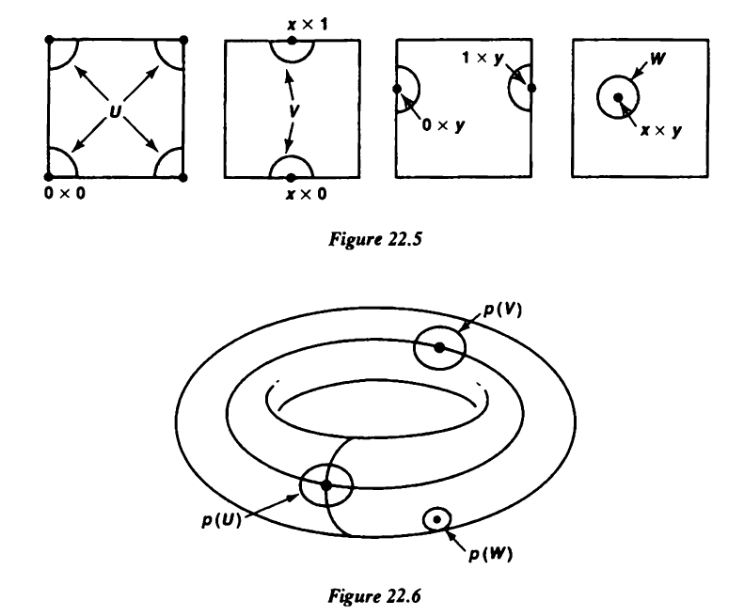
\includegraphics[width=10cm]{Torus.png}
\end{center}

Note that subspaces don't work well; if $p:X \rightarrow Y$ is a quotient map and $A$ is a subspace of $X$, there is no guarentee that $q:A \rightarrow P(A)$ is a quotient map;
the following theorem helps
\begin{theorem}
  Let $p:X \rightarrow Y$ be a quotent map, let $A$ be a subspace of $X$ that is saturated with respect to $p$, and let $q:A \rightarrow p(A)$ be a restriction of $p$:
  \begin{enumerate}[label={(\arabic*)}]
    \item If $A$ is either open or closed in $X$, the $q$ is a quotient map.
    \item If $p$ is either an open map or a closed map, then $q$ is a quotient map.
  \end{enumerate}
\end{theorem}
\begin{proof}
  Note that $p(U \cap A) \subset p(U) \cap p(A)$ for all $U,A \subset X$.
  Additionally, if $y = p(u) = p(a)$ for $u \in U$, $a \in A$, $A$ is saturated an contains $p^{-1}(p(a))$, so that $A$ cotains $u$, and $y = p(u)$, where $u \in U \cap A$.
  Hence $p(U \cap A) = p(U) \cap p(A)$.

  Take some subset $V$ of $p(A)$ for which $q^{-1}(V)$ is open.
  Suppose $A$ is open.
  Then $q^{-1}(V) = p^{-1}(V)$ is open in $A$ and $A$ is open in $X$, so $p^{-1}(V)$ is open in $X$.
  Then $V$ is open in $Y$ since $p$ is a quotient map; then $V$ is open in $p(A)$.

  Now suppose $p$ is open;
  then $q^{-1}(V) = p^{-1}(V)$ is open, so $p^{-1}(V) = U \cap A$ for some set $U$ open in $X$.
  Then,
  \[
    V = p(p^{-1}(V)) = p(U \cap A) = p(U) \cap p(A).
  \]
  Since $p(U)$ is open, $V$ is open in $p(A)$.
  The proof for closed $p$ and $A$ is similar.
\end{proof}

Note that composites of maps work well, since $p^{-1}(q^{-1}(U)) = (q \circ p)^{-1}(U)$.
However, products of maps don't work well:
the cartesian product of two quotient maps isn't necessarily a quotient map.
This is the case if either the spaces are locally compact or $p,q$ are open, forcing $p \times q$ open.

The Hausdorff condition doesn't behave well.
If each element of the partition $X^*$ is a closed subset of $X$, then $X^*$ satisfies the $T_1$ condition.
However, the Hausdorff axiom is harder.

\begin{theorem}
  Let $p:X \rightarrow Y$ be a quotient map.
  Let $Z$ be a space and let $g:X \rightarrow Z$ be a map that is constant on each set $p^{-1}(y)$ for each $y \in Y$.
  Then $g$ induces a map $f:Y \rightarrow Z$ such that $f \circ p = g$.
  The induced map $f$ is continuous iff $g$ is continuous;
  $f$ is a quotient map iff $g$ is a quotient map.
\[
  \begin{tikzcd}
    X \arrow[swap]{d}{p} \arrow{rd}{g}\\
    Y \arrow[swap]{r}{f} & Z
  \end{tikzcd}
\]
\end{theorem}
\begin{proof}
  For each $y \in Y$, $g(p^{-1}(y))$ is one point, since $g$ is constant on $p^{-1}(y)$; call this $f(y)$, and you've defined a map $f:Y \rightarrow Z$ that commutes as in the diagram.
  Suppose $U$ is open in $Z$; then $g^{-1}(U)$ is saturated in $X$ (since $g$ is constant on $p^{-1}(y)$), meaning $f^{-1}(U) = p(g^{-1}(U))$ is open for all $U$ iff $g^{-1}(U)$ is open for all $U$, i.e. $f$ is continuous iff $g$ is continuous.

  If $g$ is a quotient map, then $f$ is the composite of two quotient maps, so it is a quotient map.
  Conversely, assume $g$ is a quotient map.
  Since $g$ is surjective, so is $f$.
  Let $V \subset Z$, we show that $V$ is open in $Z$ if $f^{-1}(V)$ is open in $Y$.
  The set $p^{-1}(f^{-1}(V))$ is open because $p$ is continuous, and it is equal to $g^{-1}(V)$, so that $V$ is open in $Z$.
\end{proof}

\begin{corollary}
  Let $g:X \rightarrow Z$ be a surjective continuous map.
  Let $X^*$ be the following collection of subsets of $X$:
  \[  X^* = \cbr{g^{-1}(z) \mid z \in Z}. \]
  Give $X^*$ the quotient topology.
  \begin{enumerate}[label={(\alph*)}]
    \item The map $g$ induces a bijective continuous map $f:X^* \rightarrow Z$ which is a homeomorphism iff $g$ is a quotient map.
    \item If $Z$ is Hausdorff, so is $X^*$.
  \end{enumerate}
\end{corollary}
\begin{proof}
  The corollary gives an induced map $f$, which is continuous and surjective because $g$ is continuous and surjective.
  The partition $X^*$ separates different preimages of points in $Z$, so $f$ is bijective.
  Suppose $f$ is a homomorphism.
  Then $f$ is open, and hence a quotient map, so $g$, which is a composite of $p$ and $f$, is a quotient map.

  Suppose $g$ is a quotient map, and let $U$ be an open set in $Y$.
  Then $f(U) = g(p^{-1}(U))$, and $p^{-1}(U)$ is a saturated open set in $X$, so $f(U)$ is open and $f$ is a homeomorphism.
  If $x,y$ are points in $y$ and $f(x),f(y)$ have distinct open neighborhoods $U,V$, then $f^{-1}(U)$ and $f^{-1}(V)$ are distinct open neighborhoods of $x$ and $y$, so $X^*$ is Hausdorff if $Z$ is.
  Note: bijective quotient maps are homomorphisms.
\end{proof}

\section{Metric Space Topology}
\subsection{Properties of the Metric Space}
This may be terse;
I already covered ch2 of Rudin, so most of this is probably redundant.
\begin{definition}
  A \emph{metric} on a set $X$ is a function
  \[
    d: X \times X \rightarrow \RR
  \]
  having the following properties:
  \begin{enumerate}[label={(\arabic*)}]
    \item $d(x,y) \geq 0$ for all $x,y \in X$; equality holds iff $x = y$.
    \item $d(x,y) = d(y,x)$ for all $x,y \in X$.
    \item $d(x,y) + d(y,z) \geq d(x,z)$ for all $x,y,z \in X$.
  \end{enumerate}
\end{definition}

Given a metric $d$ on $X$, we call $d(x,y)$ the \emph{distance} between $x$ and $y$ in the metric $d$.
We will call the \emph{$\epsilon$-ball centered at $x$}
\[
  B_d(x,\epsilon) = \cbr{y \mid d(x,y) < \epsilon},
\]
and we may omit the $d$ if it's clear.

\begin{definition}
  If $d$ is a metric on the set $X$, then the collection of all $\epsilon$-balls $B_d(x,\epsilon)$ for $x \in X$ and $\epsilon > 0$ is a basis for a topology on $X$, called the \emph{metric topology} induced by $d$.
\end{definition}

To see that it's a basis, note that $x \in B(x,\epsilon)$ for the first condition.
For the second condition, let $B_1,B_2$ be basis elements and let $y \in B_1 \cap B_2$.
Then, choose $\delta_i$ so that $B(y,\delta_i) \subset B_i$, and choose $\delta \leq \min \cbr{\delta_1, \delta_2}$, so that $B(y,\delta) \subset B_1 \cap B_2$.
Using this, one can say that a set $U$ is open in the metric topology induced by $d$ iff, for each $y \in U$, there is a $\delta > 0$ such that $B_d(y,\delta) \subset U$.

\begin{definition}
  If $X$ is a topological space, $X$ is said to be \emph{metrizable} if there exists a metric $d$ on the set $X$ that induces the topology of $X$.
  A \emph{metric space} is a metrizable space $X$ together with a specific metric $d$ that gives the topology of $X$.
\end{definition}

\begin{definition}
  Let $X$ be a metric space with metric $d$.
  A subset $A$ of $X$ is said to be \emph{bounded} if there is some number $M$ such that
  \[ d(a_1,a_2) \leq M \]
  for every pair $a_1,a_2$ of points of $A$.
  If $A$ is bounded and nonempty, the \emph{diameter} of $A$ is defined to be the number
  \[ \text{diam} \, A = \sup \cbr{d(a_1,a_2) \mid a_1,a_2 \in A}. \]
\end{definition}

Boundedness of a set isn't a topological property; for any metric space $X$ with metric $d$, there exists a metric $\bar d$ that gives the topology of $X$, relative to which every subset of $X$ is bounded:

\begin{theorem}
  Let $X$ be a metric space with metric $d$.
  Define $\bar d: X \times X \rightarrow \RR$ by the equation
  \[ \bar d(x,y) = \min \cbr{d(x,y),1}. \]
  Then $\bar{d}$ is a metric that induces the same topology as $d$.
  We call $\bar{d}$ the \textbf{standard bounded metric} corresponding to $d$.
\end{theorem}
\begin{proof}
  The first two conditions are trivial.
  To check the triangle inequality, we only need to check the condition that $d(x,y) \geq 1$ or $d(y,z) \geq 1$;
  then $d(x,y) + d(y,z) \geq 1$, but $d(x,z) \leq 1$ by the bound, so the triangle inequality works.

  For equivalence, note that the collection of $\epsilon$-balls with $\epsilon < 1$ forms a basis for the metric topology, since every basis element containing $x$ contains such an $\epsilon$-ball centered at $x$.
  It follows that $d$ and $\bar d$ induce the same topology on $X$.
\end{proof}

Now we consider some familiar metrizable spaces.
\begin{definition}
  Given $x = (x_1,\dots,x_n) \in \RR^n$, we define the \emph{norm} of $x$ by the equation
  \[ \nrm{x} = (x_1^2 + \dots + x_n^2)^{1/2}; \]
  and we define the \emph{euclidean metric} $d$ on $\RR^n$ by the equation
  \[ d(x,y) = \nrm{x - y}. \]
  We define the \emph{square metric} $\rho$ by the equation
  \[ \rho(x,y) = \max \cbr{\abs{x_1 - y_1},\dots,\abs{x_n - y_n}}. \]
  The proof that $d$ is a metric is annoying and will be omitted on those grounds.
\end{definition}

To show that $\rho$ is a metric is easy: the first two conditions are trivial.
The triangle inequality for $\RR$ gives that
\[ \abs{x_i - z_i} \leq \abs{x_i - y_i} + \abs{y_i - z_i}.\]
Then, the max of the left is less than or equal to the max of the right.

We'll show that each of these metrics induces the usual topology on $\RR^n$, using the following lemma:

\begin{lemma}
  Let $d$ and $d'$ be two metrics on the set $X$, and let $\ST$ and $\ST'$ be the topologies they induce.
  Then $\ST'$ is finer than $\ST$ iff, for each $x \in X$ and each $\epsilon > 0$, there exists a $\delta > 0$ such that
  \[ B_{d'}(x,\delta) \subset B_d(x,\epsilon).\]
\end{lemma}
\begin{proof}
  This is immediate from the lemma that says that we need a basis element $B'$ with $x \in B' \subset B_d(x,\epsilon)$. 
\end{proof}

\begin{theorem}
  The topologies on $\RR^n$ generated by the euclidean metric $d$ and the square metric $\rho$ are the same as the product topology on $\RR^n$.
\end{theorem}
\begin{proof}
  Let $x,y$ be two points of $\RR^n$.
  Note that
  \[ \rho(x,y) \leq d(x,y) \leq \sqrt{n} \rho(x,y) .\]
  Then, use the lemma, that $B_d(x,\epsilon) \subset B_\rho(x,\epsilon)$, and that $B_\rho(x,\epsilon) \subset B_d(x,\epsilon/\sqrt{n})$; the two are equivalent.

  Note that the basic element of a basis for the product topology on $\RR^n$ has the form $B = (a_1,b_1)\times\dots\times(a_n,b_n)$.
  Let $x = (\frac{b_1 + a_1}{2},\dots,\frac{b_n + a_n}{2})$ be the center of $B$, and let $\delta = \min \cbr{\abs{\frac{b_1 - a_1}{2}},\dots,\abs{\frac{b_1 - a_1}{2}}}$.
  Then $B_\rho(x,\delta) \subset B$, so the topology generated by $\rho$ is finer than the standard topology.
  Since every basis element for the topology generated by $\rho$ is a basis element for the product topology, the other direction also holds, making all three topologies equivalent.
\end{proof}

We want to be able to generalize this to $\RR^\omega$, but this leads to infinite sums and sups which do not always converge or exist.
However, we can use the bounded euclidean metric on $\RR$ to generalize the square metric to $\RR^J$ for arbitrary $J$:

\begin{definition}
  Given an index set $J$, and given points $x = (x_\alpha), y = (y_\alpha)$ in $\RR^J$, we'll define the following metric:
  \[ \bar \rho (x,y) = \sup \cbr{ \bar d(x_\alpha,y_\alpha) \mid \alpha \in J}, \]
  where $\bar d$ is the standard bounded metric on $\RR$.
  It's easy to check that $\bar \rho$ is a metric.
  We call this the \emph{uniform metric} on $\RR^J$, and the topology it induces is called the \emph{uniform topology}.
\end{definition}

\begin{theorem}
  The uniform topology on $\RR^J$ is finer than the product topology and coarser than the box topology;
  these three topologies are all different if $J$ is infinite.
\end{theorem}
\begin{proof}
  Suppose that we are given a point $x = (x_\alpha)$ contained in a product topology basis element $\prod U_\alpha$.
  Let $\alpha_1,\dots,\alpha_n$ be the indices where $U_\alpha \neq \RR$, and let $\epsilon_i > 0$ be such that $B_{\bar d}(x_{\alpha_i},\epsilon_i) \subset U_{\alpha_i}$.
  Let $\epsilon \leq \min \cbr{\epsilon_i}$.
  Then, $B_{\bar \rho}(x,\epsilon) \subset \prod U_\alpha$, so the uniform topology is finer than the product topology.
  Furthermore, if $J$ is infinite and $0 < \epsilon < 1$, $B_{\bar \rho}(x,\epsilon)$ is open in the uniform topology but not in the box topology, so it is strictly finer.

  Note that any basis element for the uniform topology $B_{\bar \rho}(x,\epsilon)$ is a basis element for the box topology $\prod (x_\alpha - \epsilon,x_\alpha + \epsilon)$.
  However, if $J$ is infinite, it contains a subset indexed by $\NN$; call these $\alpha_n$ for $n \in \NN$.
  Then, if $U_{\alpha_n} = (-1/n,1/n)$ (and $U_\alpha = X_\alpha$ for non-indexed $\alpha$), no $\epsilon > 0$ gives a $B_{\bar \rho}(x,\epsilon)$ contained in $\prod U_\alpha$ by the Archimedian property.
  Hence the inclusion is strict for infinite $J$.
\end{proof}

In the case where $J$ is infinite, we want to know whether $\RR^J$ is metrizable in either the box or product topology.
It turns out this is only the case when $J$ is countable and $\RR^J$ has the product topology.

\begin{theorem}
  Let $\bar d$ be the standard bounded metric, and for $x,y \in \RR^\omega$, define
  \[ D(x,y) = \sup \cbr{\frac{\bar d(x_i,y_i)}{i}}.\]
  Then $D$ is a metric that induces the product topology on $\RR^\omega$.
\end{theorem}
\begin{proof}
  All properties but the triangle inequality for $D$ being a metric are obvious.
  Note that 
  \[
    \frac{\bar d(x_i,z_i)}{i} 
    \leq \frac{\bar d(x_i,y_i)}{i} + \frac{\bar d(y_i,z_i)}{i}
    \leq D(x,y) + D(y,z),
  \]
  so that $D(x,z) \leq D(x,y) + D(y,z)$.

  We'll show that $D$ gives the product topology.
  First, let $U$ be open in the metric topology and let $x \in U$.
  Choose some $B_D(x,\epsilon) \subset U$, and choose $N$ such that $1/N < \epsilon$.
  Then, we can make the following basis element for the product topology:
  \[    
    V = \prn{x_1 - \epsilon,x_1 + \epsilon} \times \dots \times \prn{x_N - \epsilon,x_N + \epsilon} \times \RR \times \RR \times \dots .
  \]
  We assert that $V \subset B_D(x,\epsilon)$: given any $y \in \RR^\omega$, 
  that $d(x_i,y_i) < \omega$ is clear for all $i \leq N$.
  For all $i \geq N$, $\frac{\bar d(x_i,y_i)}{i} \leq \epsilon$ since $\bar d$ is bounded by 1, giving that $V \subset B_D(x,\epsilon)$, and The product topology is finer than the metric topology.

  Conversely, consider a basis element $U = \prod U_i$, where $U_i$ is a proper subset of $\RR$ for $i = \alpha_i,\dots,\alpha_n$.
  Choose $\epsilon_{\alpha_i}$ such that $B_d(x_{\alpha_i},\epsilon_{\alpha_i}) \subset U_{\alpha_i}$ for each $i$, and choose $\epsilon < \min \cbr{\epsilon_{i}/i \mid i = \alpha_i,\dots,\alpha_n}$.
  Then, $B_D(x,\epsilon) \subset U$, so the topologies are equal.
\end{proof}

Note some important properties of metric spaces:
\begin{theorem}
  Suppose $(X,d)$ is a metric space.
  \begin{enumerate}[label={(\alph*)}]
    \item If $A$ is a subspace of $X$, the restriction of $d$ to $A \times A$ is a metric for the topology of $A$.
    \item $X$ is Hausdorff.
    \item Countable products of metrizable spaces are metrizable.
  \end{enumerate}
\end{theorem}
\begin{proof}
  (a) is obvious.
  If $x,y$ are distinct points of $X$, and $\epsilon = \frac{d(x,y)}{2}$, then $B_d(x,\epsilon)$ and $B_d(y,\epsilon)$ are disjoint, giving (b).
  The proof of (c) is analogous to the proof that $\RR^\omega$ is metrizable, replacing intervals with balls wherever needed.
\end{proof}

\subsection{Continuous Functions on Metric Spaces}
\begin{theorem}
  Let $f:X \rightarrow Y$ and let $X$ and $Y$ be spaces with metrics $d_X$ and $d_Y$.
  Then continuity of $f$ is equivalent to the requirement that, given $x \in X$ and $\epsilon > 0$, there exists $\delta > 0$ such that
\[ d_X(x,y) < \delta \implies d_Y(f(x),f(y)) < \epsilon.\]
\end{theorem}
\begin{proof}
  Suppose that $f$ is continuous.
  Then, for each $B(f(x),\epsilon)$, there exists a neighborhood $U$ of $x$ with $f(U) \subset B(f(x),\epsilon)$;
  choose $\delta$ so that $B(x,\delta) \subset U$.

  Conversely, suppose the $\epsilon-\delta$ condition is satisfied, and let $V$ be open in $Y$.
  Let $x \in f^{-1}(V)$;
  there is an $\epsilon$-ball $B(f(x),\epsilon)$ contained in $V$, and by the condition, there is a $\delta$-ball centered at $x$ such that $f(B(x,\delta)) \subset B(f(x),\epsilon) \subset V$.
  Then $B(x,\delta)$ is a neighborhood of $x$ contained in $f^{-1}(V)$, so that $f^{-1}(V)$ is open.
\end{proof}

We'll go through many theorem's which have one direction that requires the space to be metrizable:

\begin{lemma}
  Let $X$ be a topological space and let $A \subset X$.
  If there is a sequence of points of $A$ converging to $x$, then $x \in \bar A$.
  The converse holds if $X$ is metrizable.
\end{lemma}
\begin{proof}
  If there is a sequence $a_n \rightarrow x$, then any neighborhood of $x$ has infinite intersection with $A$, so $x$ is a limit point of $A$, giving $x \in \bar A$.
  Conversely, suppose $X$ is metrizable and $x \in \bar A$.
  Then, for each $n$, choose some $a_n \in A \cap B(x,1/n)$.
  If $U$ is a neighborhood of $x$, there must be some basis element $B(x,\epsilon)$ contained in $U$; then $a_n \in B(x,\epsilon) \subset U$ for all $n > 1/\epsilon$, so $a_n \rightarrow x$.
\end{proof}

\begin{theorem}
  Let $f:X \rightarrow Y$.
  If the function $f$ is continuous, then for every convergent sequence $x_n \rightarrow x$ in $X$, the sequence $f(x_n)$ converges to $f(x)$.
  The converse holds if $X$ is metrizable.
\end{theorem}
\begin{proof}
  Suppose $f$ is continuous.
  Then, for every neighborhood $V$ of $f(x)$, there is a neighborhood $U$ of $x$ which maps into $V$.
  Since $U$ contains infinitely many points of $x_n$, $f(U)$ contains infinitely many points of $f(x_n)$, giving $f(x_n) \rightarrow f(x)$.

  Suppose $X$ is metrizable and for every convergent sequence $x_n \rightarrow x$ in $X$, $f(x_n) \rightarrow f(x)$.
  Suppose $x \in \bar A$.
  Then, there is a sequence $x_n$ of points of $A$ converging to $x$, so $f(x_n)$ converges to $f(x)$, giving a nonzero intersection of any neighborhood of $f(x)$ with $f(A)$, meaning $f(\bar A) \subset \overline{f(a)}$ and $f$ is continuous.
\end{proof}

Note: the lemma (and hence the theorem) didn't actually use metrizability; they used the collection $B_d(x,1/n)$ of balls about $x$.
We say that a space $X$ has a \emph{countable basis at the point $x$} if there is a countable collection $\cbr{U_n}_{n \in \ZZ_+}$ of neighborhoods of $x$ such that any neighborhood $U$ of $x$ contains at least one of the sets $U_n$.
We say that a space $X$ that has a countable basis at each of its points satisfies the \emph{first countability axiom}.
This is enough to prove the lemma, replacing $B_d(x,1/n)$ with $U_1 \cap \dots \cap U_n$.
Any metrizable space satisfies the first countability axiom.

\begin{theorem}
  If $X$ is a topological space, and if $f,g:X \rightarrow \RR$ are continuous functions, then $f+g$, $f - g$, and $f \cdot g$ are continuous.
  If $g(x) \neq 0$ for all $x$, then $f/g$ is continuous.\qed
\end{theorem}

\begin{definition}
  Let $f_n:X \rightarrow Y$ be a sequence of functions from the set $X$ to the metric space $(Y,d)$.
  We say that the sequence $(f_n)$ \emph{converges uniformly} to the function $f:X \rightarrow Y$ if, given $\epsilon > 0$, there exists an integer $N$ such that
  \[  d(f_n(x),f(x)) < \epsilon \]
  for all $n > N$ and all $x \in X$.
\end{definition}

Uniformity of convergence depends not only on the topology of $Y$, but also on its metric.

\begin{theorem}
  {\normalfont (Uniform limit theorem).}
  Let $f_n:X \rightarrow Y$ be a sequence of continuous functions from the topological space $X$ to the metric space $(Y,d)$.
  If $f_n \rightarrow f$ uniformly, then $f$ is continuous.
\end{theorem}
\begin{proof}
  Let $V$ be open in $Y$ and let $x_0 \in f^{-1}(V)$.
  Choose $\epsilon$ so that $B(y_0,\epsilon) \subset V$.
  Choose $N$ so that $d(f_n(x),f(x)) < \epsilon/3$.
  By continuity, there is a neighborhood of $U$ of $x_0$ that maps into $B(f_n(x_0),\epsilon/3)$ through $f$; for all $x \in U$, 
  \[
    d(f(x),f(x_0)) \leq d(f(x),f_n(x)) + d(f_n(x),f_n(x_0)) + d(f_n(x_0),f(x)) < \epsilon.
  \]
  Then, $f(U) \subset V$ so $f$ is continuous.
\end{proof}

The naming of uniform convergence is suggestive:
consider the space $\RR^X$ of all functions $f:X \rightarrow \RR$ in the uniform metric $\bar \rho$.
It isn't hard to see that a sequence of functions $f_n:X \rightarrow \RR$ converges uniformly to $f$ iff it converges as elements of the metric space $(\RR^X,\bar \rho)$.

Let's consider some counterexamples.
We'll show that $\RR^\omega$ in the box topology is not metrizable because the sequence lemma doesn't hold.
Let $A$ be the subset of $\RR^\omega$ with positive coordinates and $)$ be the origin.
$0 \in \bar A$; however, if $a_n = (x_1n,x_2n,\dots)$ the set
\[
  B = (-x_{11},x_{11}) \times (-x_{22},x_{22}) \times \dots
\]
contains $0$ and none of $a_n$, so $a_n$ fails to converge to $0$.

We'll show that an uncountable product of $\RR$ with itself isn't metrizable.
Let $A$ be the subset of $\RR^J$ consisting of all points $(x_\alpha)$ such taht $x_\alpha = 1$ for all but finitely many values of $\alpha$, and let $0$ be the origin.
To see that $0 \in \bar A$, take any basis element containing $0$, and set all of the indices where $U_\alpha = \RR$ to 1 and everything else to $0$ to find an intersection.
Let $a_n$ be a sequence of points of $A$; let $J_n$ be the subset of $J$ where the $\alpha$th coordinate of $a_n$ is different from 1.
The union of $J_n$ is countable, so there is an index $\beta$ outside of the union.
Then, the open set $\pi_\beta^{-1}((-1,1))$ is a neighborhood of 0 that contains none of $a_n$, so $a_n$ fails to converge to 0.
\end{document}
